\documentclass{standalone}
\usepackage{tikz}
\usepackage{ctex,siunitx}
\setCJKmainfont{Noto Serif CJK SC}
\usepackage{tkz-euclide}
\usepackage{amsmath}
\usetikzlibrary{patterns, calc}
\usetikzlibrary {decorations.pathmorphing, decorations.pathreplacing, decorations.shapes,}
\begin{document}
\small
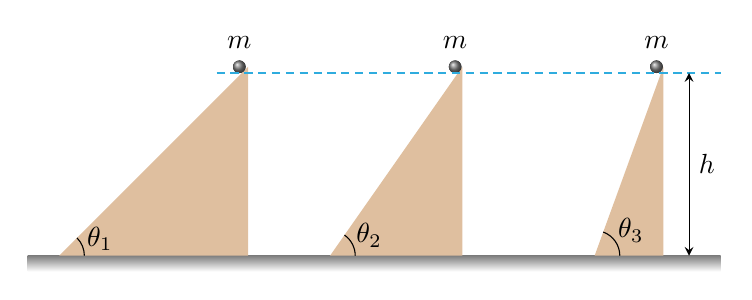
\begin{tikzpicture}[>=stealth,scale=0.8]
  \fill [top color =gray, bottom color=white](-7,-.25) rectangle (4,0);
  % \coordinate(A)at(4,3);
  \tkzDefPoints{-6.5/0/A,-2.2/0/B,2.0/0/C,3.5/0/X,-2/3/Y,4/3/Z}
  \tkzDefShiftPoint[A](45:1){A'}
  \tkzDefShiftPoint[B](55:1){B'}
  \tkzDefShiftPoint[C](70:1){C'}
  \tkzInterLL(A,A')(Y,Z)\tkzGetPoint{A''}
  \tkzInterLL(B,B')(Y,Z)\tkzGetPoint{B''}
  \tkzInterLL(C,C')(Y,Z)\tkzGetPoint{C''}
  \fill [brown!50](A)--(A'')--(A''|- 0,0)--cycle;
  \fill [brown!50](B)--(B'')--(B''|- 0,0)--cycle;
  \fill [brown!50](C)--(C'')--(C''|- 0,0)--cycle;
  \fill [ball color=gray,semithick]([xshift=-1.4mm]A'') circle (.1)node[above=1mm]{$m$};
  \fill [ball color=gray,semithick]([xshift=-1.15mm]B'') circle (.1)node[above=1mm]{$m$};
  \fill [ball color=gray,semithick]([xshift=-1.1mm]C'') circle (.1)node[above=1mm]{$m$};
  \tkzLabelAngle[pos=0.7](X,A,A'){$\theta_1$}
  \tkzLabelAngle[pos=0.7](X,B,B'){$\theta_2$}
  \tkzLabelAngle[pos=0.7](X,C,C'){$\theta_3$}
  \tkzMarkAngle[size=4mm](X,A,A')
  \tkzMarkAngle[size=4mm](X,B,B')
  \tkzMarkAngle[size=4mm](X,C,C')
  \draw [densely dashed, cyan!80!gray] (-4,2.9)--(4,2.9);
  \draw [thin,<->](3.5,2.9)--(3.5,0)node[midway,right]{$h$};
\end{tikzpicture}
\end{document}